% Class tree of the functions of CAP (src/core/Math/Functions) and the classes they depend on.
% Used by the paper (section "Functions", figure fig:functions) and by the Doxygen documentation (Function.hpp, with
% IMAGE_PATH of src/Doxyfile including docs/paper/figures).
%   pdflatex FunctionClasses.tex                                          -> FunctionClasses.pdf (paper)
%   pdftoppm -r 200 -png -singlefile FunctionClasses.pdf FunctionClasses  -> FunctionClasses.png (Doxygen)
%   pdftocairo -svg FunctionClasses.pdf FunctionClasses.svg               -> FunctionClasses.svg
\documentclass[tikz,border=2pt]{standalone}
\usepackage[scaled=0.92]{helvet}
\usetikzlibrary{arrows.meta,shapes.multipart,positioning}
\renewcommand{\familydefault}{\sfdefault}
\definecolor{abstract}{HTML}{D6E4F5}
\definecolor{concrete}{HTML}{EEF4FB}
\definecolor{group}{HTML}{EEEEEE}
\definecolor{depend}{HTML}{FFF8E6}
\definecolor{dependline}{HTML}{8A6D3B}
\begin{document}
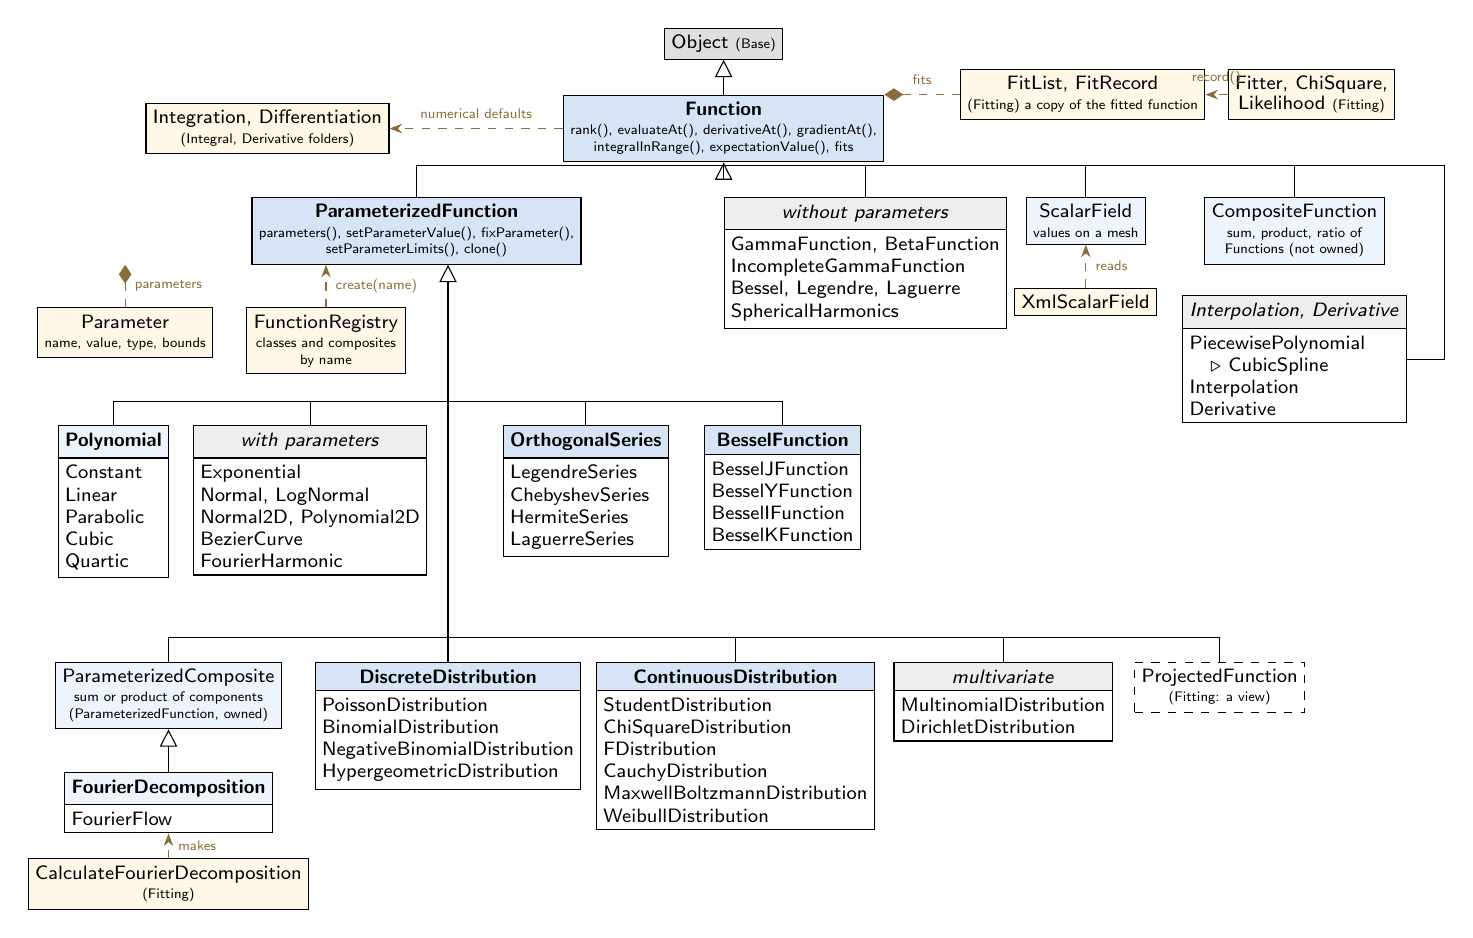
\begin{tikzpicture}[
    font=\scriptsize,
    cls/.style={draw, fill=concrete, align=center, inner sep=2.5pt, anchor=north},
    abs/.style={cls, fill=abstract},
    dep/.style={cls, fill=depend},
    fam/.style={draw, rectangle split, rectangle split parts=2, rectangle split part fill={#1,white},
                rectangle split part align={center,left}, inner sep=2.5pt, anchor=north, align=left},
    note/.style={font=\tiny},
    inherit/.style={-{Triangle[open,length=2.2mm,width=2.2mm]}, thin},
    bus/.style={thin},
    uses/.style={dashed, dependline, -{Stealth[length=1.6mm]}, thin},
    owns/.style={dashed, dependline, {Diamond[length=2.4mm,width=1.6mm]}-, thin},
    lbl/.style={font=\tiny, text=dependline},
  ]

  % ---------------------------------------------------------------- base classes
  \node[cls, fill=gray!25] (Object) at (8.6,0) {Object \tiny(Base)};
  \node[abs] (Function) at (8.6,-0.85) {\textbf{\textit{Function}}\\[-1pt]\tiny rank(), evaluateAt(), derivativeAt(), gradientAt(),\\[-2pt]\tiny integralInRange(), expectationValue(), fits};
  \draw[inherit] (Function.north) -- (Object.south);

  % ---------------------------------------------------------------- derived from Function
  \node[abs] (PF) at (4.7,-2.15)
    {\textbf{\textit{ParameterizedFunction}}\\[-1pt]
     \tiny parameters(), setParameterValue(), fixParameter(),\\[-2pt]
     \tiny setParameterLimits(), clone()};
  \node[fam=group] (Special) at (10.4,-2.15)
    {\textit{without parameters}\nodepart{two}GammaFunction, BetaFunction\\IncompleteGammaFunction\\
     Bessel, Legendre, Laguerre\\SphericalHarmonics};
  \node[cls] (ScalarField) at (13.2,-2.15) {ScalarField\\[-1pt]\tiny values on a mesh};
  \node[cls] (CompositeFunction) at (15.85,-2.15) {CompositeFunction\\[-1pt]\tiny sum, product, ratio of\\[-2pt]\tiny Functions (not owned)};
  \draw[inherit] (PF.north |- 0,-1.75) -| (Function.south);
  \draw[bus] (PF.north) -- (PF.north |- 0,-1.75) -- (CompositeFunction.north |- 0,-1.75) -- (CompositeFunction.north);
  \draw[bus] (Special.north) -- (Special.north |- 0,-1.75);
  \draw[bus] (ScalarField.north) -- (ScalarField.north |- 0,-1.75);
  \node[fam=group] (Tools) at (15.85,-3.4)
    {\textit{Interpolation, Derivative}\nodepart{two}PiecewisePolynomial\\\quad$\triangleright$ CubicSpline\\Interpolation\\Derivative};
  \draw[bus] (Tools.east) -| (17.75,-1.75) -- (CompositeFunction.north |- 0,-1.75);

  % ---------------------------------------------------------------- derived from ParameterizedFunction (1)
  \def\busA{-4.75}
  \node[fam=concrete] (Polynomial) at (0.85,-5.05)
    {\textbf{Polynomial}\nodepart{two}Constant\\Linear\\Parabolic\\Cubic\\Quartic};
  \node[fam=group] (Simple) at (3.35,-5.05)
    {\textit{with parameters}\nodepart{two}Exponential\\Normal, LogNormal\\Normal2D, Polynomial2D\\BezierCurve\\FourierHarmonic};
  \node[fam=abstract] (Series) at (6.85,-5.05)
    {\textbf{\textit{OrthogonalSeries}}\nodepart{two}LegendreSeries\\ChebyshevSeries\\HermiteSeries\\LaguerreSeries};
  \node[fam=abstract] (Bessel) at (9.35,-5.05)
    {\textbf{\textit{BesselFunction}}\nodepart{two}BesselJFunction\\BesselYFunction\\BesselIFunction\\BesselKFunction};
  \def\trunk{5.1}
  \draw[inherit] (\trunk,\busA) -- (\trunk,-2.15 |- PF.south);
  \draw[bus] (Polynomial.north) -- (Polynomial.north |- 0,\busA) -- (Bessel.north |- 0,\busA) -- (Bessel.north);
  \draw[bus] (Simple.north) -- (Simple.north |- 0,\busA);
  \draw[bus] (Series.north) -- (Series.north |- 0,\busA);

  % ---------------------------------------------------------------- derived from ParameterizedFunction (2)
  \def\busB{-7.75}
  \node[cls] (Composite) at (1.55,-8.05) {ParameterizedComposite\\[-1pt]\tiny sum or product of components\\[-2pt]\tiny (ParameterizedFunction, owned)};
  \node[fam=abstract] (Discrete) at (5.1,-8.05)
    {\textbf{\textit{DiscreteDistribution}}\nodepart{two}PoissonDistribution\\BinomialDistribution\\
     NegativeBinomialDistribution\\HypergeometricDistribution};
  \node[fam=abstract] (Continuous) at (8.75,-8.05)
    {\textbf{\textit{ContinuousDistribution}}\nodepart{two}StudentDistribution\\ChiSquareDistribution\\FDistribution\\
     CauchyDistribution\\MaxwellBoltzmannDistribution\\WeibullDistribution};
  \node[fam=group] (Multivariate) at (12.15,-8.05)
    {\textit{multivariate}\nodepart{two}MultinomialDistribution\\DirichletDistribution};
  \node[cls, fill=white, dashed] (Projected) at (14.9,-8.05) {ProjectedFunction\\[-1pt]\tiny (Fitting: a view)};
  \draw[bus] (\trunk,\busA) -- (\trunk,\busB);
  \draw[bus] (Composite.north) -- (Composite.north |- 0,\busB) -- (Projected.north |- 0,\busB) -- (Projected.north);
  \draw[bus] (Continuous.north) -- (Continuous.north |- 0,\busB);
  \draw[bus] (Multivariate.north) -- (Multivariate.north |- 0,\busB);
  \draw[bus] (Discrete.north) -- (Discrete.north |- 0,\busB);

  \node[fam=concrete] (Fourier) at (1.55,-9.45) {\textbf{FourierDecomposition}\nodepart{two}FourierFlow};
  \draw[inherit] (Fourier.north) -- (Composite.south);

  % ---------------------------------------------------------------- classes the functions depend on
  \node[dep] (Parameter) at (1.0,-3.55) {Parameter\\[-1pt]\tiny name, value, type, bounds};
  \node[dep] (Registry) at (3.55,-3.55) {FunctionRegistry\\[-1pt]\tiny classes and composites\\[-2pt]\tiny by name};
  \draw[owns] (PF.south -| Parameter.north) -- node[lbl, right]{parameters} (Parameter.north);
  \draw[uses] (Registry.north) -- node[lbl, right]{create(name)} (PF.south -| Registry.north);

  \node[dep, anchor=west] (FitRecord) at (11.6,-0.85) {FitList, FitRecord\\[-1pt]\tiny (Fitting) a copy of the fitted function};
  \node[dep, anchor=west] (Fitter) at (15.0,-0.85) {Fitter, ChiSquare,\\[-1pt]Likelihood \tiny (Fitting)};
  \node[dep, anchor=east] (Tools2) at ([xshift=-2.2cm]Function.west) {Integration, Differentiation\\[-1pt]\tiny (Integral, Derivative folders)};
  \draw[uses] (Function.west) -- node[lbl, above]{numerical defaults} (Tools2.east);
  \draw[owns] (Function.east |- FitRecord.west) -- node[lbl, above]{fits} (FitRecord.west);
  \draw[uses] (Fitter.west) -- node[lbl, above]{record()} (FitRecord.east);

  \node[dep] (Xml) at (13.2,-3.3) {XmlScalarField};
  \draw[uses] (Xml.north) -- node[lbl, right]{reads} (ScalarField.south);

  \node[dep] (CalcFourier) at (1.55,-10.55) {CalculateFourierDecomposition\\[-1pt]\tiny (Fitting)};
  \draw[uses] (CalcFourier.north) -- node[lbl, right]{makes} (Fourier.south);
\end{tikzpicture}
\end{document}
